%%%%%%%%%%%%%%%%%%%%%%%%%%%%%%%%%%%%%%%%%%%%%%%%%%%%%%%%%%%%%%%
%
% Welcome to Overleaf --- just edit your LaTeX on the left,
% and we'll compile it for you on the right. If you open the
% 'Share' menu, you can invite other users to edit at the same
% time. See www.overleaf.com/learn for more info. Enjoy!
%
%%%%%%%%%%%%%%%%%%%%%%%%%%%%%%%%%%%%%%%%%%%%%%%%%%%%%%%%%%%%%%%
\documentclass[aspectratio=169]{beamer}
\usepackage{tikz}
\usepackage{amsmath}
\usepackage{amssymb}
\usepackage{graphicx}
\usepackage{stmaryrd}
\usepackage{listings}
\usetikzlibrary{decorations.pathreplacing,calligraphy}
\usetheme{Copenhagen}
\usecolortheme{default}
\beamertemplatenavigationsymbolsempty
\setbeamertemplate{footline}[frame number]
\title[Final presentation for CS4280] %optional
{Final presentation for LCI}
\subtitle{Simple and precise static analysis of untrusted Linux kernel extensions}
\author[]
{Giulio Piva}



\date[VLC 2021] % (optional)
{UniPI, December 2023}

% Use a simple TikZ graphic to show where the logo is positioned


%End of title page configuration block
%------------------------------------------------------------
%The next block of commands puts the table of contents at the 
%beginning of each section and highlights the current section:

\AtBeginSection[]
{
  \begin{frame}
    \frametitle{Table of Contents}
    \tableofcontents[currentsection]
  \end{frame}
}
%------------------------------------------------------------
\begin{document}
\frame{\titlepage}
%---------------------------------------------------------
%Highlighting text
\begin{frame}
  \frametitle{eBPF}

  \begin{figure}
    \centering
    % \includegraphics[width=0.2\textwidth]{EBPF_logo.png}

  \end{figure}

  \begin{itemize}
    \item eBPF is a technology that allows the extension of Kernel functionalities
          without actually modifying the Kernel code.
    \item Users applications are not allowed to access kernel memory
    \item Advanced applications require to analyze kernel events:
          Networking, Security, observability, debugging, etc...
    \item \textbf{untrusted kernel extensions}: Still need to account for malicious code
  \end{itemize}
  \begin{figure}
    \centering
    % \includegraphics[width=0.2\textwidth]{cilium.png}
    % \includegraphics[width=0.2\textwidth]{falco.png}
    % \includegraphics[width=0.2\textwidth]{deepflow.png}
  \end{figure}
\end{frame}


\begin{frame}{eBPF compilation process}
  \begin{figure}
    \centering
    \includegraphics[width=\textwidth]{images/ebpf-overview.png}
  \end{figure}
  \begin{itemize}
    \item eBPF program can be written in a supported high level language (C++, Rust, Go, etc...)
    and then compiled to eBPF bytecode IR
    \item Verifier checks that the program doesn't violate security properties
    \item Verification done at compile time to avoid runtime overhead
  \end{itemize}
\end{frame}

\begin{frame}[fragile]{Memory safety}

  eBPF program cannot access memory locations outside of the bounds of its assigned memory areas
  \begin{lstlisting}[frame=single]
int main(){
  pid_t pid = getpid();
  // privilege-escalation
  ebpf_overwrite_uid(pid)
  ebpf_overwrite_gid(pid)
  ebpf_overwrite_euid(pid)
  // spawn a shell with root privileges
  system("/bin/sh");
  return 0;
}
\end{lstlisting}
\end{frame}

\begin{frame}{Information flow security}
  \begin{itemize}
    \item eBPF programs cannot leak information about the kernel to the userspace
    \item Reading uninitialized memory areas is dangerous
    \item e.g It might be used to defeat KASLR and obtain addresses of vulnerable kernel functions to
          be used in a buffer overflow attack.
  \end{itemize}
  \centering


\end{frame}

\begin{frame}{Memory areas}
  eBPF program has access to three memory areas:
  \begin{itemize}
    \item Stack: private memory area used as operand stack
    \item Packet: variable-size memory area which stores an incoming/outgoing network packet
    \item Shared memory: for inter-process communication
  \end{itemize}
\end{frame}

\begin{frame}{Prevail: a new eBPF verifier}
  The current verifier has two main drawbacks:
  \begin{itemize}
    \item Not guaranteed to be sound
    \item Lack of precision
  \end{itemize}
  The authors of this paper propose a new verifier based on \textit{Abstract Interpretation} to tackle these
  problems
\end{frame}

\begin{frame}{Language syntax}
  $$
    \begin{aligned}
       & \text { cmd }::=w:=E\left|w:=_{s z} * p\right| * p:=_{s z} x \\
       & \mid \text { assume(B) } \mid w:=\operatorname{shared} K     \\
       & E::=K|x| x+y \mid x-y                                        \\
       & B ::=x=y|x \neq y| x \leq y                                  \\
       &
    \end{aligned}
  $$
\end{frame}

\begin{frame}{Operational semantics}
  The semantics of a program is defined as a transition relation which checks that executing the command is safe using the safe () predicate before continuing according to the transition relation of safe commands:
  $$
    \langle c m d, \sigma\rangle \Rightarrow_{\xi} \begin{cases}\sigma^{\prime} & \mathrm{Safe}(c m d, \sigma) \wedge\langle c m d, \sigma\rangle \Rightarrow \sigma^{\prime} \\ \xi & \text { otherwise }\end{cases}
  $$
\end{frame}

\begin{frame}{Machine state}
  $$\sigma = (e, \mu, \zeta)$$
  $$
    \begin{aligned}
       & \mathcal{R}=\text { Shared } \cup\{\text {ctx, stk, pkt, num, inv}\}                  \\
       & e \in \text { Env } =\text { Register } \rightarrow(\mathcal{R} \times \mathbb{Z})    \\
       & \mu \in \text { Mem } =\text { Cell } \hookrightarrow(\mathcal{R} \times \mathbb{Z})  \\
       & \zeta \in \text { Format }=2^{\text {Address }}                                       \\
       & \sigma \in \text { State }=\text { Env } \times \text { Mem } \times \text { Format } \\
       &
    \end{aligned}
  $$
  \begin{itemize}
    \item e maps a register names to their content
    \item $\mu$ maps memory cells to their content
    \item $\zeta$ keeps track of addresses in thew stack which stores num values
  \end{itemize}

\end{frame}

\begin{frame}{Safe predicate}
  $$ Safe(cmd, \sigma ) = Safe_{inv} (cmd, \sigma ) \And Safe_{cmd} (\sigma) $$
  $$Safe_{inv}(cmd, \sigma) = inv \notin \{ {e_{p(x)} | x \in ReadRegs(cmd)\}}$$
  \begin{itemize}
    \item $Safe_{inv}$ states that no register mentioned
          in a statement whose value is read can hold an invalid value:
    \item ReadRegs(cmd) denotes the set of registers whose
          values are read in cmd.
  \end{itemize}
\end{frame}

\begin{frame}{Safe predicate for memory safety}
  \begin{itemize}
    \item Pointers are stored as offset from the beginning of the region they are pointing to, given by $\mathcal{R}$
    \item Load and write can access a variable number of bytes (subscript sz)
    \item Checks that p is actually a pointer
    \item Ensures that pointers are not leaked to other memory areas with the store operation

  \end{itemize}

  $$
    \begin{aligned}     &
                   \operatorname{Safe}_{w:=_{s z} * p}(\sigma)=\text { inbounds }\left(e_\rho(p), e_n(p), s z\right) \wedge e_\rho(p) \neq \text { num }                                                                                     \\ &
                   \mathrm{Safe}_{* p:=s z}(\sigma)=\operatorname{inbounds}\left(e_\rho(p), e_n(p), s z\right) \wedge e_\rho(p) \neq \text { num }                                                                                           \\ &
                   \qquad \qquad \qquad \qquad \qquad \qquad \wedge e_\rho(x) \neq \mathrm{num} \rightarrow e_\rho(p)=\mathrm{stk}                                                                                                           \\ &
                   \text { inbounds }(R, a, s z)= \left\{\begin{array}{l}0 \leq a \leq e_{n} (\text{data\_end})-sz \quad R=\mathrm{pkt} \\ 0 \leq a \leq \text {sizeof}(R)-sz \quad \text { otherwise }\end{array}\right. \\ &
    \end{aligned}
  $$
\end{frame}

\begin{frame}{Safe predicate for information flow security}
  \begin{itemize}
    \item Prevents sum of pointers
    \item Avoids leaking information regarding the layout of the kernel
  \end{itemize}

  $$
    \begin{aligned}
      \text { Safe }_{\text {assume }(x \bowtie y)}(\sigma)=e_\rho(x)=e_\rho(y) \vee e(x)=(\text { num, } 0) \\
      \vee e(y)=(\text { num, } 0)                                                                           \\
    \end{aligned}
  $$
  $$
    \text { Safe }_{\text {assume }(x \leq y)}(\sigma)=e_\rho(x)=e_\rho(y)
  $$
  $$
    \operatorname{Safe}_{w:=E}(\sigma)= \begin{cases}e_\rho(x)=\text { num } \vee e_\rho(y)=\text { num } & E=x+y \\ e_\rho(x)=e_\rho(y) \vee e_\rho(y)=\text { num } & E=x-y \\ \text { true } & \text { otherwise }\end{cases}
  $$
\end{frame}

\begin{frame}{Transition relation of safe commands}
  $$
    \begin{aligned}
       & \langle\mathrm{w}:=\mathrm{K}, \sigma\rangle \Rightarrow(e[w \mapsto(\text { num, } K)], \mu, \zeta)                                             \\
       & \langle\mathrm{w}:=\mathrm{x}, \sigma\rangle \Rightarrow(e[w \mapsto e(x)], \mu, \zeta)                                                          \\
       & \langle\mathrm{w}:=\mathrm{x}+\mathrm{y}, \sigma\rangle \Rightarrow\left(e\left[w \mapsto\left(R, e_n(x)+e_n(y)\right)\right], \mu, \zeta\right) \\
       & \quad \text { where } R=\text { if }\left(e_\rho(x)=\text { num then } e_\rho(y) \text { else } e_\rho(x)\right.                                 \\
       & \langle\mathrm{w}:=\mathrm{x}-\mathrm{y}, \sigma\rangle \Rightarrow\left(e\left[w \mapsto\left(R, e_n(x)-e_n(y)\right)\right], \mu, \zeta\right) \\
       & \quad \text { where } R=\text { if }\left(e_\rho(x)=e_\rho(y)\right) \text { then num else } e_\rho(x)
    \end{aligned}
  $$
  $$
    \begin{array}{lr}
      \langle\text { assume }(\mathrm{x}=\mathrm{y}), \sigma\rangle \Rightarrow \sigma      & \text { if } e_n(x)=e_n(y) \wedge e_\rho(x)=e_\rho(y)         \\
      \langle\text { assume }(\mathrm{x} \neq \mathrm{y}), \sigma\rangle \Rightarrow \sigma & \text { if } e_n(x) \neq e_n(y) \vee e_\rho(x) \neq e_\rho(y) \\
      \langle\text { assume }(\mathrm{x} \leq \mathrm{y}), \sigma\rangle \Rightarrow \sigma & \text { if } e_n(x) \leq e_n(y)
    \end{array}
  $$
  \centering{...}
\end{frame}

\begin{frame}{Store operation}
  \begin{itemize}
    \item A (safe) store to the stack removes any segment overlapping with the written memory cell
    \item Only memory cells of the stack are tracked
  \end{itemize}
  \begin{align*}
     & \left\langle * \mathrm{p}:={ }_{s z} x, \sigma\right\rangle \Rightarrow\left(e, \mu^{\prime}, \zeta^{\prime}\right) \quad \hspace{3cm} \text{if } e_\rho(p)=\text{ stk } \\
     & \hspace{0.4cm} \text{ where }\left(\mu^{\prime}, \zeta^{\prime}\right)=\operatorname{Store}\left(\mu, \zeta,\left(e_n(p), s z\right), e(x)\right)                        \\
     & \left\langle * \mathrm{p}:=_{s z} x, \sigma\right\rangle \Rightarrow \sigma \quad \hspace{4.3cm} \text{if } e_\rho(p) \neq \text{ stk }                                  \\
  \end{align*}

  \begin{minipage}{0.1\textwidth}

    \begin{align*}
       & \text { Store }(\mu, \zeta, c,(R, n))=\left(\mu^{\prime}[c \mapsto(R, n)], \zeta^{\prime}\right)                                    \\
       & \quad \text { where } \quad \overline{c}=\{i \in \mathbb{Z} \mid c \leq i<c+n\}                                                     \\
       & \quad \mu^{\prime}=\mu\left[c_o \mapsto \perp \mid c_o \in \text { Cell } \wedge \overline{c_o} \cap \bar{c} \neq \emptyset\right]  \\
       & \quad \zeta^{\prime}=\text { if }(R=\operatorname{num}) \text { then }(\zeta \cup \bar{c}) \text { else }(\zeta \backslash \bar{c}) \\
    \end{align*}
  \end{minipage}
  \vline
  \begin{minipage}{0.12\textwidth}
    $$*p=_4 13$$

    $$*p=_2 8 $$
  \end{minipage}%
  \hspace*{0cm}
  \begin{minipage}{0.05\textwidth}
    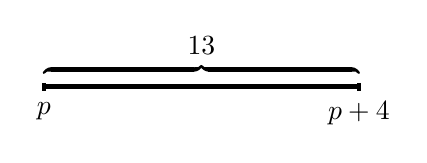
\begin{tikzpicture}[ultra thick]
      \def\x{4}
      \def\tick{0.05}
      \draw (0,0) -- (\x,0);
      \draw (0,\tick) -- ++(0,-2*\tick) node[below] {$p$};
      \draw (2,\tick)  node[above=6pt] {13};
      \draw (\x,\tick) -- ++(0,-2*\tick) node[below] {$p+4$};
      \draw [decorate,
        decoration = {calligraphic brace,raise=5pt}] (0,0) --  (4,0);
    \end{tikzpicture}
    \vspace{-0.5cm}
    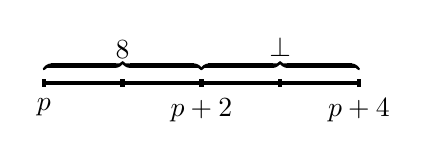
\begin{tikzpicture}[ultra thick]
      \def\x{4}
      \def\tick{0.05}

      \draw (0,0) -- (\x,0);
      \draw (0,\tick) -- ++(0,-2*\tick) node[below] {$p$};
      \draw (1,\tick) -- ++(0,-2*\tick) node[above=6pt] {8};
      \draw (0.5*\x,\tick) -- ++(0,-2*\tick) node[below] {$p+2$};
      \draw (3,\tick) -- ++(0,-2*\tick) node[above=7pt] {$\perp$};
      \draw (\x,\tick) -- ++(0,-2*\tick) node[below] {$p+4$};

      \draw [decorate,
        decoration = {calligraphic brace,raise=5pt}] (2,0) --  (4,0);

      \draw [decorate,
        decoration = {calligraphic brace,raise=5pt}] (0,0) --  (2,0);
    \end{tikzpicture}
  \end{minipage}


\end{frame}

\begin{frame}{Load operation}
  \begin{itemize}
    \item Reading an uninitialized cell which is supposed to contain a pointer is dangerous: it might contain
    a sensible address!
    \item Conversely, reading an uninitialized numeric cell is considered safe as it is initialized with a default value
  \end{itemize}
  \begin{align*}
     & \left\langle\mathrm{w}:=_{s z} * \mathrm{p}, \sigma\right\rangle \Rightarrow(e[w \mapsto v], \mu, \zeta) \quad \text{ if } e_\rho(p)=\text{stk}              \\
     & \qquad \text { where } v \in \operatorname{Load}\left(\mu, \zeta,\left(e_n(p), s z\right)\right)                                                             \\
     & \left\langle\mathrm{w}:=_{s z} * \mathrm{p}, \sigma\right\rangle \Rightarrow(e[w \mapsto v], \mu, \zeta) \quad \quad \text{ if } e_\rho(p) \neq \text{ stk } \\
     & \qquad \text { where } v=(\operatorname{num}, \beta) \wedge \beta \in \mathbb{Z}
  \end{align*}

  $$
    \begin{aligned}
       & \operatorname{Load}(\mu, \zeta, c)=\text { if }(c \in \operatorname{dom}(\mu)) \text { then }\{\mu(c)\} \text { else }\left(\left\{R^{\prime}\right\} \times \mathbb{Z}\right) \\
       & \quad \text { where } R^{\prime}=\text { if }(\bar{c} \subseteq \zeta) \text { then num else inv }
    \end{aligned}
  $$
\end{frame}

\begin{frame}{Static analysis}
  \begin{itemize}
    \item The abstract interpretation algorithm conservatively over-approximates this semantics.
    \item If the analyzer manages to verify that a program never aborts, it effectively
          establishes that it is safe to execute the program in the kernel.
    \item Abstraction performed in two steps
  \end{itemize}
\end{frame}

\begin{frame}{First step: Abstracting shared regions}
  $$
    \begin{aligned}
       & \hspace{1cm} \mathcal{T}_{Shared} = \{\text{K} | \text{(w := shared  K)} \in P \}                                                                 \\
       & \hspace{1cm} \mathcal{T}=\mathcal{T}_{\text {Shared }} \cup\{\text { ctx, stk, pkt, num, inv }\}                                                  \\
       & \left(e_\tau, \mu_\tau\right) \in \text { Tags } =(\text { Register } \rightarrow \mathcal{T}) \times(\text { Cell } \hookrightarrow \mathcal{T}) \\
       & \left(e_n, \mu_n\right) \in \text { Values }=(\text { Register } \rightarrow \mathbb{Z}) \times(\text { Cell } \hookrightarrow \mathbb{Z})        \\
       &                                                                                                                                                   \\
       & \vspace{1cm} \hspace{1cm} \widehat{\sigma} \in \widehat{\text { State }}=\text { Tags } \times \text { Values } \times \text { Format }           \\
       &
    \end{aligned}
  $$

  \begin{itemize}
    \item Rearrengement of the machine state notation
    \item Replaces the (unbounded) set of shared region
          identifiers found in R with the (bounded) set of the sizes K
          which appear in shared K commands in the program P
    \item Shared regions size still tracked precisely $=>$ no adaptations needed for memory safety checking
  \end{itemize}
\end{frame}

\begin{frame}{Safe predicate update}
  \begin{itemize}
    \item Pointers to the shared area cannot be substracted or compared
          since it is not possible to distinguish them anymore
  \end{itemize}

  $$
    \begin{aligned}
       & \operatorname{Safe}_{w:=x-y}(\widehat{\sigma})=  e_\tau(x)=e_\tau(y) \wedge e_\tau(y) \notin \mathcal{T}_{\text {Shared }}  \vee e_\tau(y)=\text { num. } \\
       & \text { Safe }_{\text {assume }(x \leq y)}(\widehat{\sigma})=  e_\tau(x)=e_\tau(y) \wedge e_\tau(y) \notin \mathcal{T}_{\text {Shared }} .                \\
    \end{aligned}
  $$
\end{frame}

\begin{frame}{Abstract domain}
  $$\mathbb{V}=\text { Register } \cup \text { Cell } $$
  $$ \Sigma^{\sharp} = \mathcal{D}_T ( \mathbb{V} ) \times \mathcal{D}_N (\mathbb{V}) \times 2^{\text {Address }} \times 2^{\text {Cell }}$$
  $$\sigma^{\sharp}=(\theta, d, \zeta, \delta) \in \Sigma^{\sharp} $$
  $$ \llbracket c m d \rrbracket^{\sharp}(\sigma^{\sharp}) \Rightarrow_{\xi} \begin{cases}\sigma^{\prime \sharp} & \mathrm{Safe^{\sharp}}(c m d, \sigma^{\sharp}) \wedge\llbracket c m d^{\sharp} \rrbracket (\sigma^{\sharp}) \Rightarrow \sigma^{\prime \sharp} \\ \xi & \text { otherwise }\end{cases} $$

  \begin{itemize}
    \item Parametric abstract domains for tags ($\mathcal{D}_T$) and values ($\mathcal{D}_N$)
    \item Requirements for $\mathcal{D}_T$: $\sqcup_T$, variable assignments operations, assignments of constants sets of abstract
          tags to variables
    \item Requirements for $\mathcal{D}_N$: $\sqcup_N$, assignments of arithmetic and boolean expressions to variables, havoc
    \item $\delta$ is used to track the set of cells \textbf{definitely} present in memory and fail safely if needed
  \end{itemize}
\end{frame}

\begin{frame}{Abstract operations}
  $$
    \llbracket w := \mathrm{K} \rrbracket^{\sharp}(\theta, d, \zeta, \delta)= (\llbracket w= \{num\} \rrbracket_{T}^{\sharp}(\theta),\llbracket w=K \rrbracket_{N}^{\sharp}(d),\zeta,\delta)
  $$

  $$
    \llbracket w := x \rrbracket^{\sharp}(\theta, d, \zeta, \delta)= (\llbracket w= \theta(x) \rrbracket_{T}^{\sharp},\llbracket w=x \rrbracket_{N}^{\sharp},\zeta,\delta)
  $$

  $$
    \llbracket w := x + y \rrbracket^{\sharp}(\theta, d, \zeta, \delta) = (\llbracket w=R \rrbracket^{\sharp}_{T},\llbracket w=x+y \rrbracket_{N}^{\sharp},\zeta,\delta)
  $$
  $$ R= \text{if} \thickspace \theta(x) = { \{num \}} \thickspace \text{then} \thickspace \theta(y) \thickspace \text{else} \thickspace \theta(y)$$

  \begin{itemize}
    \item Just delegate the operations for calculating the new tags and values to
    chosen abstract domains to produce the new abstract machine state
  \end{itemize}
\end{frame}


\begin{frame}{Abstract store and abstract load}
  \noindent
  \begin{minipage}{0.55\textwidth}
    \begin{figure}
      \centering
      \includegraphics[width=\textwidth]{loadstore.png}
    \end{figure}
  \end{minipage}
  \begin{minipage}{0.40\textwidth}
    distinguish between two cases
    \begin{itemize}
      \item pointer still tracked precisely
      \item pointer is not tracked precisely
    \end{itemize}
    havoc = forget everything about the variable

  \end{minipage}
\end{frame}



\begin{frame}{Benchmarks}
  \begin{minipage}{0.45\textwidth}
    \begin{figure}
      \includegraphics[width=0.8\textwidth]{analysis-time.png}
    \end{figure}
  \end{minipage}
  \begin{minipage}{0.5\textwidth}
    \begin{figure}
      \includegraphics[width=0.7\textwidth]{memory-usage.png}
    \end{figure}
  \end{minipage}
  \begin{itemize}
    \item Verifier tested on a set of 192 programs
    \item "Biased" benchmark: only programs that pass the verifier
    \item Precision depends on the choice of the abstract domains
          \begin{itemize}
            \item Interval: Fails to verify 64 programs
            \item Zone: Fails to verify 1 program
            \item Octagon: Fails to verify 1 program
          \end{itemize}
  \end{itemize}
\end{frame}

\begin{frame}{}
  \centering{Questions?}
\end{frame}
\end{document}
